\chapter{Geological background}

To understand more about bank erosion, you must have knowledge about the soil profile of the delta region. This chapter intends to combine all the information found, regarding the soil, in our investigation area.

\section{The geology of a delta}
A delta is a landscape formed at the mouth of a river where the water eventually runs into the ocean. At a delta is the velocity of the water decreasing which gives floating particles in the delta the change to settle. Among this floating particles are gravels, sands and clays. Whereas they are descending in particle size. The particles are formed by erosion of stone. The origin of the particles is in the Parana river are the Andes mountains. 
Besides that are deltas also characterized by high vegetation growth. When this vegetation dies will the organic material due to pressure change into peat. So, in a delta it's expected to find relatively soft soils (sands) and very soft soils (clay and peat). 

\section{Borehole}
One of the things that is found about the subsoil is a borehole. This borehole is done in the area of the port of Ibicuy. From this data is made the following soil profile \autocite{amatoESTRATIGRAFIACUATERNARIASUBSUELO2009};

\begin{figure}[H]
    \centering
    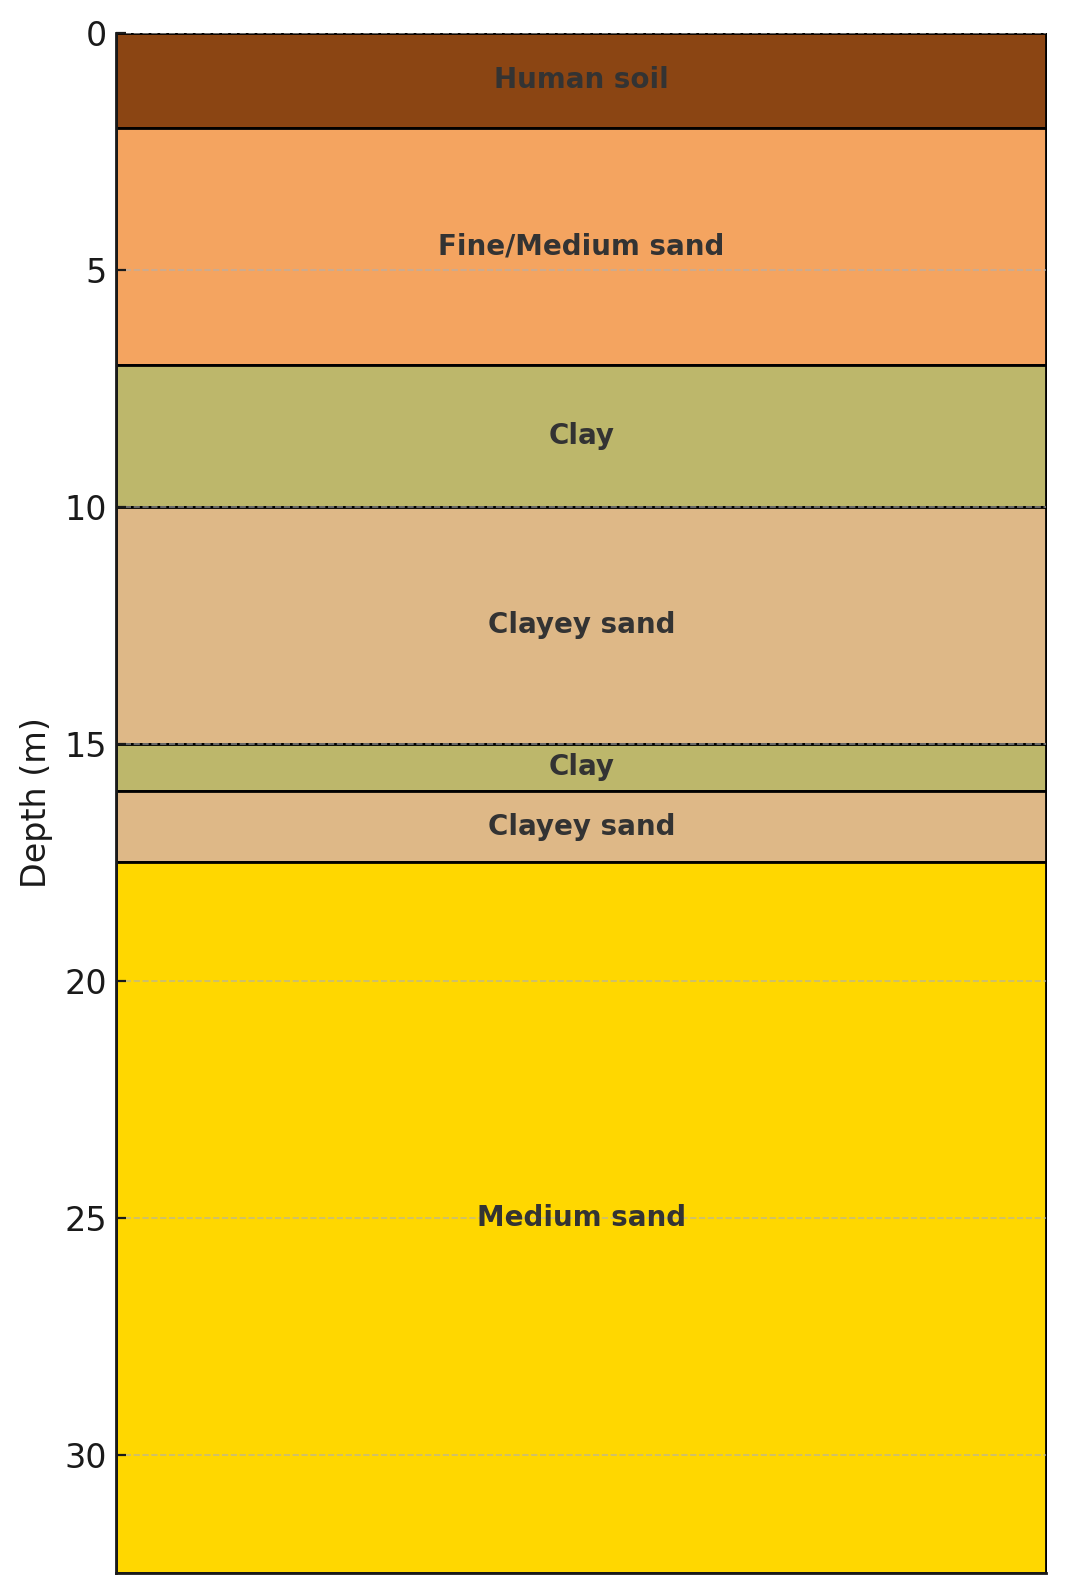
\includegraphics[width=0.45\linewidth]{figures//ch9/Bodemprofiel.png}
    \caption{Borehole profile}
    \label{fig:placeholder}
\end{figure}

\section{Geological cross section}
A study was conducted that led to a morphological map of the Paraná delta. In the study, for two cross sections a more detailed geological profile was made, one of which is relevant to the area of interest. The cross section along with the area is interest is shown in figure \ref{fig:crosssectiongeo}.

\begin{figure}[H]
    \centering
    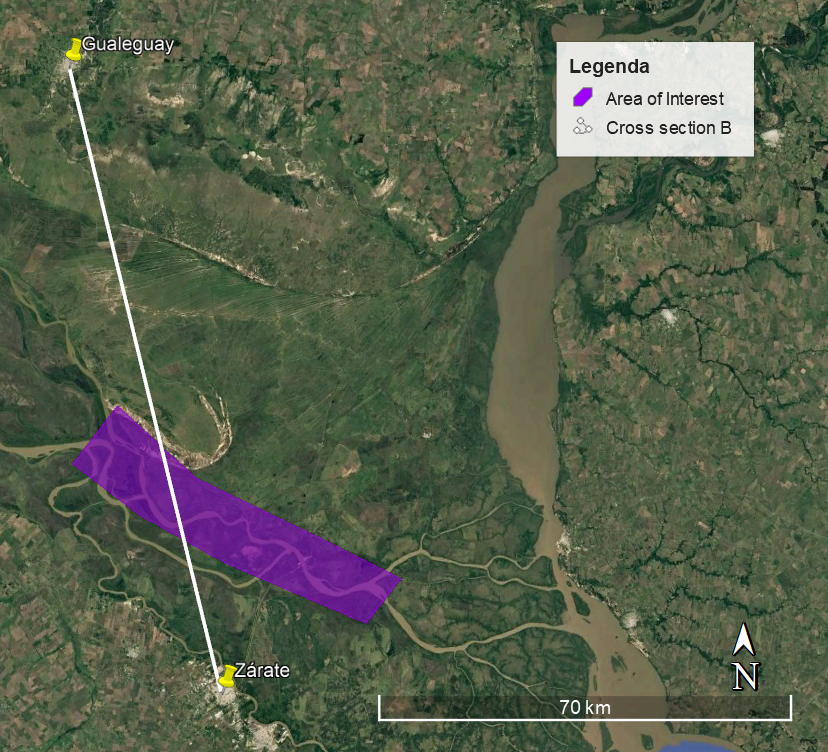
\includegraphics[width=0.75\linewidth]{figures/ch9/CrossSectionB.png}
    \caption{Cross section}
    \label{fig:crosssectiongeo}
\end{figure}

The geological profile of the cross section is shown in figure \ref{fig:geolprofile}. As can be seen in the figure, the taken cross section was around 80 km long. Of this, 15 km falls inside the area of interest, this zone is marked with purple.

\begin{figure}[H]
    \centering
    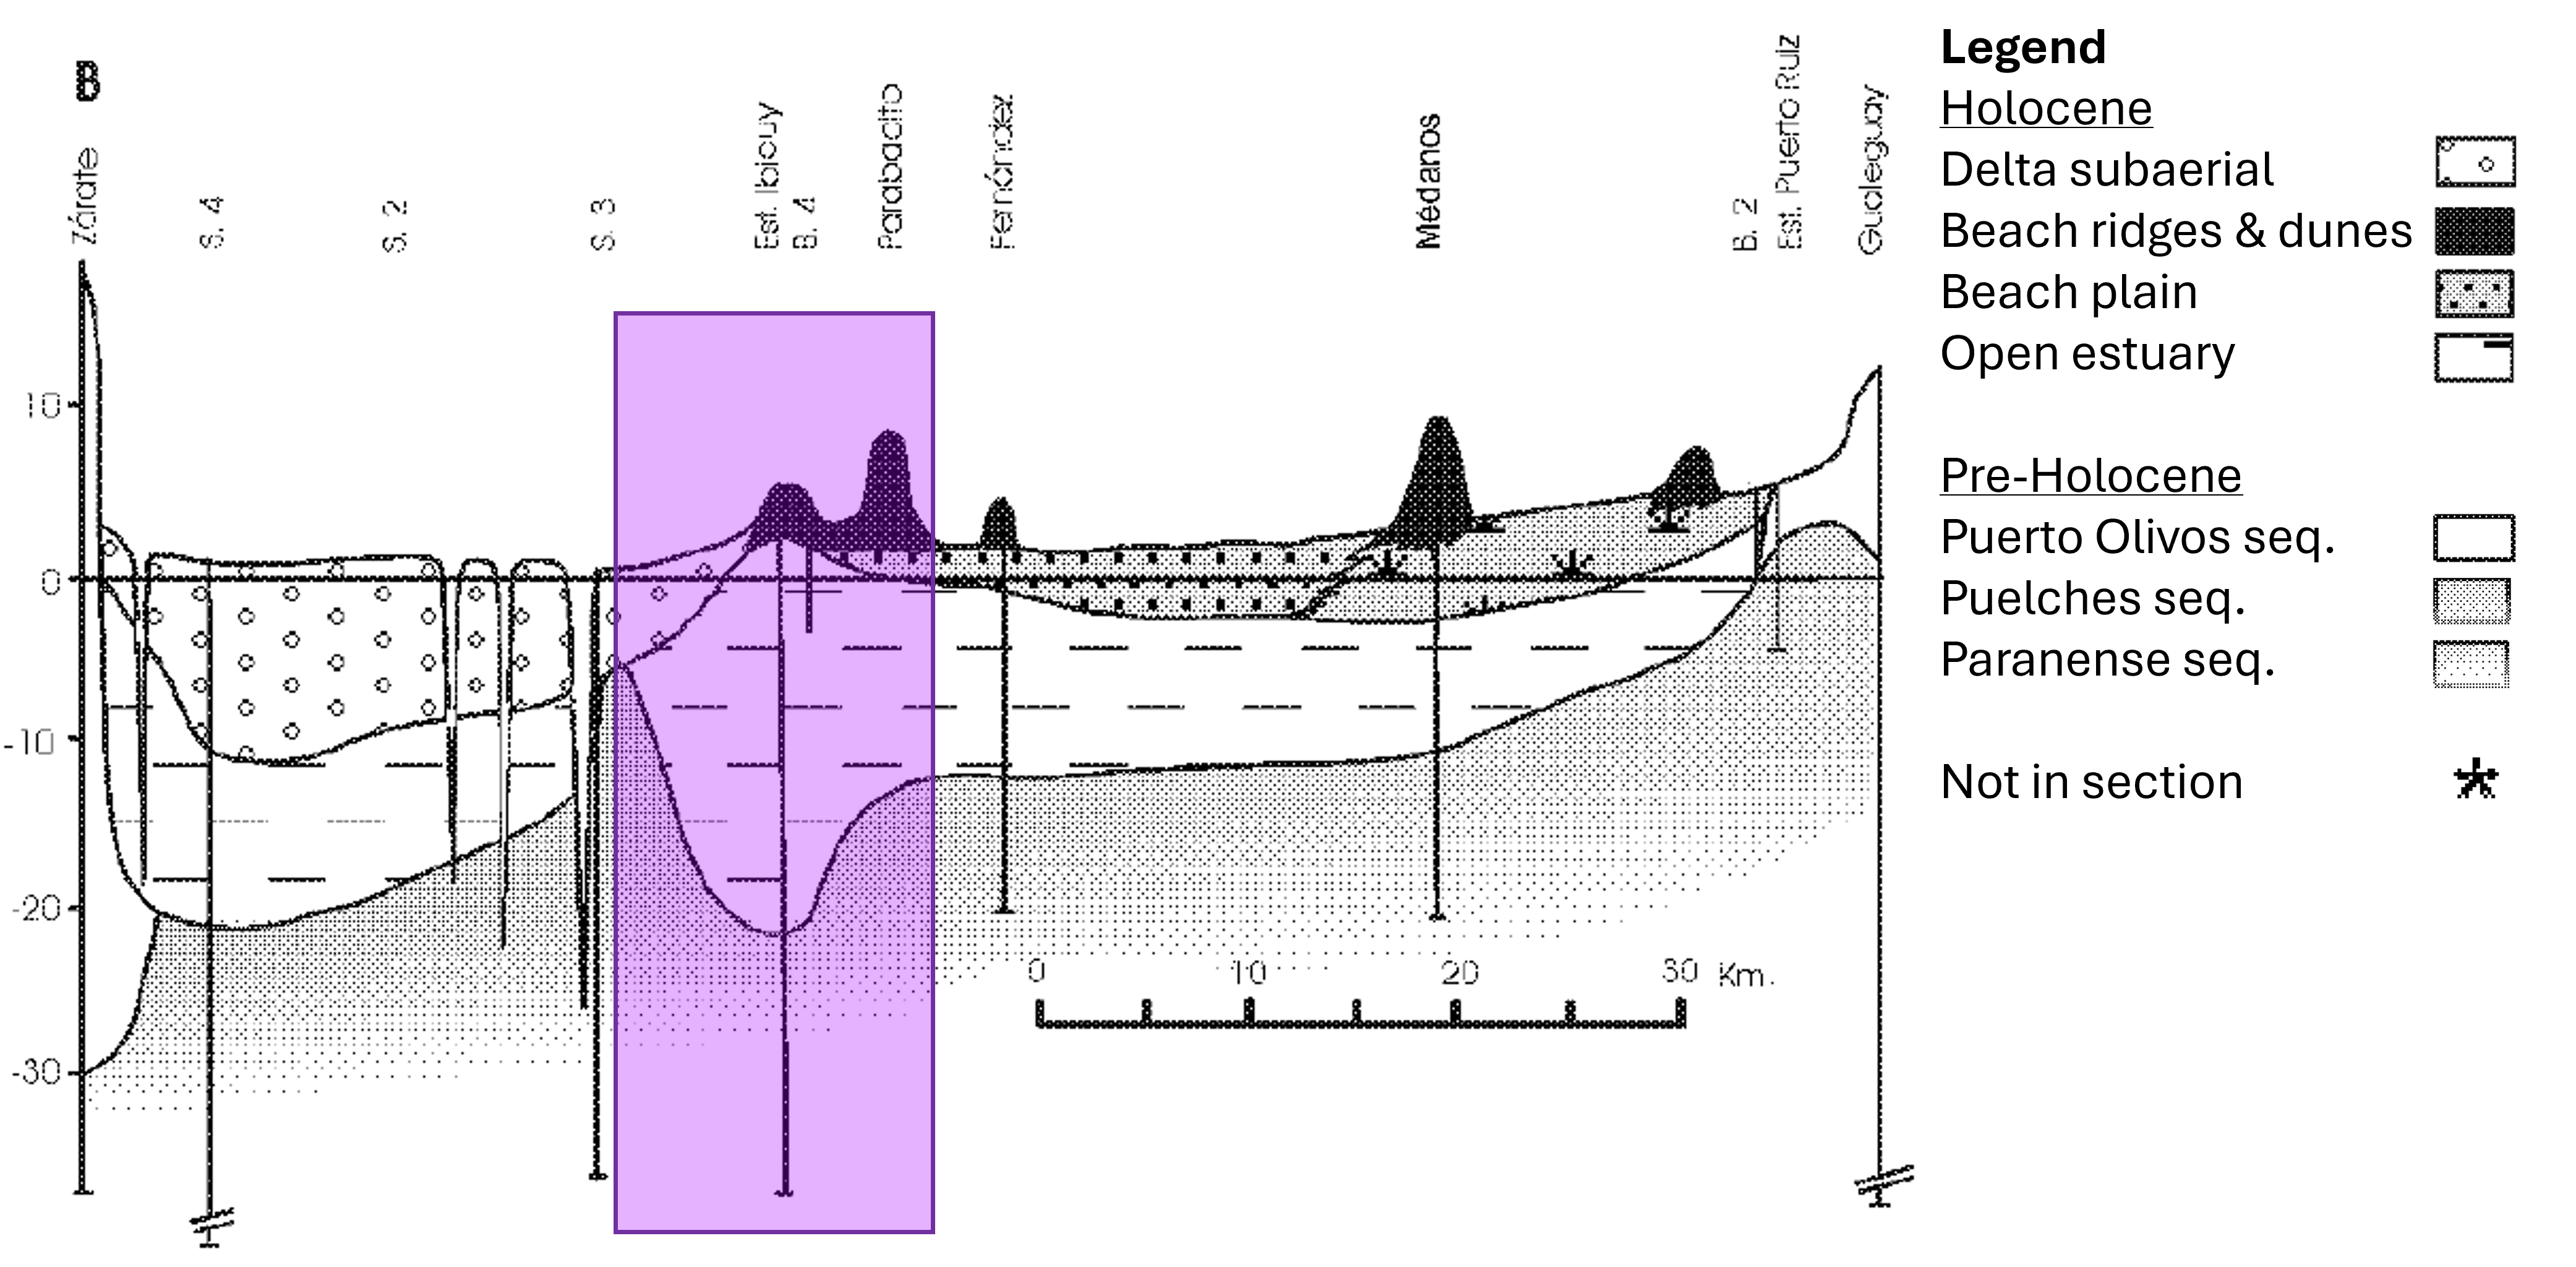
\includegraphics[width=1\linewidth]{figures/ch9/CrossSectionBResults.png}
    \caption{Geological profile of cross section}
    \label{fig:geolprofile}
\end{figure}

In figure \ref{fig:geolprofile}, the first kilometers of the purple zone are especially of interest since these are located near the river. The following layers can be identified in this area.

\subsection{Subaerial facies}
The subaerial facies of the Paraná Delta developed through the deposition of silty-sandy sediments delivered mainly by the Paraná Guazú and Paraná de las Palmas. These deposits, subject to coastal processes and occasional flooding from the Río de la Plata, occur at elevations between 2 m and sea level, with a maximum thickness of 12 m. This is the layer that is drained.

Mineralogical analyses show a predominance of quartz with minor plagioclase and K-feldspar, plus heavy minerals such as magnetite, hematite, garnet, zircon, tourmaline, and others, generally well-rounded except zircon, which preserves crystal form \textbf{1949}. The age of the unit is debated: radiocarbon dates suggest origin dates between -150 BC and 180 AD, while other authors propose a later origin around 700–750 AD.

\subsection{Open estuary}
The open estuary sediments were deposited during postglacial sea-level rise and were formed at the freshwater–saltwater interface during the upstream migration of the maximum salinity gradient, which filled the Río de la Plata river valley.

These are olive-green clays to silty clays with thin fine-sand layers, scattered or concentrated shell beds, and fossil content confirming estuarine conditions. The unit is dated to the Holocene, with its base at ~6670 +/- 100 years BP, occurring between –22 and –0 m and reaching up to 20 m thick.

\subsection{Paranense depositional sequence}
During the Miocene, large portions of present-day Argentina, Uruguay, Paraguay, southern Brazil, and eastern Bolivia were covered by the Paranense Sea. This was a shallow sea that advanced from the Atlantic into the interior of South America. Its waters left behind extensive marine sediments and fossils and this layer is now known as the Paranense depositional sequence.

It is composed mainly of siliciclastic sandstones, mudstones, and bioclastic beds, with thicknesses ranging from a few meters in outcrop to over 100 m. The lower part has mud-dominated offshore deposits with marine fossils, while the upper part shows sandier shoreface. Strontium isotope ages constrain the unit to the Late Miocene (ca. 9.5–6.7 Ma).